\RequirePackage{mmap}
\documentclass[12pt]{article}
\usepackage[utf8]{inputenc}
\usepackage{geometry}
\geometry{
  margin=1in,
}
\usepackage{amsmath,amsthm,amssymb, listings, color}
\usepackage{mathtools}
\usepackage{changepage}% http://ctan.org/pkg/changepage
\usepackage{enumitem}
\usepackage{csquotes}
\usepackage{fancyhdr}
\usepackage[T1]{fontenc}
\usepackage{titlesec}
\usepackage[absolute]{textpos}
\usepackage[hidelinks]{hyperref}
\usepackage{fontspec}
\setmainfont{Latin Modern Roman}
%% \usepackage{setspace}
%% \doublespacing

\newcommand\defeq{\stackrel{\mathclap{\normalfont\mbox{\scriptsize def}}}{=}}
\newtheorem{theorem}{Theorem}[section]
\newtheorem{corollary}{Corollary}[theorem]
\newtheorem{lemma}[theorem]{Lemma}
\newtheorem{innercustomgeneric}{\customgenericname}
\providecommand{\customgenericname}{}
\newcommand{\newcustomtheorem}[2]{%
  \newenvironment{#1}[1]
  {%
   \renewcommand\customgenericname{#2}%
   \renewcommand\theinnercustomgeneric{##1}%
   \innercustomgeneric
  }
  {\endinnercustomgeneric}
}

\newcustomtheorem{customthm}{Theorem}
\newcustomtheorem{customlemma}{Lemma}
\newcustomtheorem{customdef}{Definition}

\newcommand{\istart}[1]{\underline{\textit{#1}}\\}
\newcommand{\idetail}[1]{\footnotesize\textbf{\emph{#1}}\normalsize}
\newcommand{\mapto}{\rightarrow}
\newcommand{\bR}{\mathbb{R}}

\setlength{\parindent}{0.25in}
\setlength{\parskip}{0.5em}

\newif\ifextra
\extrafalse

\title{}

\pagenumbering{arabic}

\begin{document}
\pagestyle{fancy}
\fancyhf{} % sets both header and footer to nothin
\cfoot{\thepage}
\renewcommand{\headrulewidth}{1pt}
\lhead{\fontsize{10}{12} \selectfont CSE 599: Convex Optimization and Geometry (Prof. Yin Tat Lee)\\\textbf{Summary of Lecture 1} }
\rhead{\fontsize{10}{12} \selectfont Kaiyu Zheng\\ \today}

This series of lecture summaries is to extract the key theorems and ideas from the lecture notes. I do not understand them all, but at least I condense the knowledge and do not need to read the lengthy lecture notes again.

\section{Convex sets and functions}
\begin{enumerate}
  \item \istart{Convex set} $K$ is convex set if for $x,y\in K$, $0\leq t\leq 1$, $tx+(1-t)y\in K$.
  \item \istart{Polyhedron} $K=\{x\in\bR^n: Ax\leq b\}$ is a polyhedron. A polyhedron doesn't have to be boudned.
  \item \istart{Polyhedron is as general as convex sets}
    For convex set $K\in\bR^n$ and $y\notin K$, $\exists \theta\in\bR^n$ such that $\theta^Ty\geq\max_{x\in K}\theta^Tx$. If $K$ is closed (bounded), the inequality is strict.
  \item \istart{A convex set is intersection of half spaces} Any closed convex set $K$ can be written as the intersection of half spaces as
    \[
      K = \bigcap_{\theta\in\bR^n}\{x: \theta^Tx \leq \max_{y\in K} \theta^Ty\}
     \]
    \idetail{Note} Inside the set notation, $\theta$ is fixed. And because $\theta$ can be arbitrary from $\bR^n$, you can always find a half space that covers $K$. See Figure \ref{fig:halfspace}.
    \begin{figure}[h]
      \centering
      \includegraphics[scale=1]{figs/halfspace}
      \caption{Example region $\{x: \theta^Tx\leq\max_{y\in K}\theta^Ty\}$ to be intersected with (dashed)}
      \label{fig:halfspace}
    \end{figure}    
  \item \istart{Convex function} $f:\bR^n\mapto\bR\cup\{+\infty\}$ is convex if for all $x,y\in\bR^n$ and $0\leq t\leq 1$,
    $$f(tx+(1-t)y)\leq tf(x)+(1-t)f(y)$$
  \item \istart{Epigraph}
    The epigraph of convex function $f(x)$ is the ``region above $f$'':
    $$\text{epi}f\defeq\{(x,t)\in\bR^n\times\bR: t\geq f(x)\}$$
  \item \istart{Relation between epigraph and convex function}
    A function $f$ is convex if and only if epi$f$ is a convex set.
  \item \istart{Convexity test via first-order differentiation}
    Let $f$ be a continuously differentiable function. Then $f$ is convex if and only if
    $$f(y)\geq f(x)+(\nabla f(x))^T(y-x)$$
  \item \istart{Convexity test via Hessian}
    Let $f$ be a twice continuously differentiable function on $\bR^n$. Then $f$ is convex if and only if for all $x\in\bR^n$,
    $$\nabla^2f(x)\succeq 0$$
    \idetail{Note} The Hessian $\nabla^2f(x)$ is an $n\times n$ matrix defined by $(\nabla^2f(x))_{ij}=\frac{\partial^2 f}{\partial x_i\partial x_j}$. The notation $A\succeq 0$ means matrix $A$ is positive-semidefinite.
  \item \istart{Convex optimization problem} A convex optimization problem is of the form
    $$ min_{x\in\bR^2} f(x)$$
    where $f$ is convex.
  \item \istart{Minimizer of convex function} Let $f$ be a continuously differentiable convex function. Then $x$ is the minimizer of $f$ if and only if $\nabla f(x)=0$.
  
\end{enumerate}
%% \bibliography{references}
%% \bibliographystyle{plain}

\end{document}

